\documentclass[12pt,listsleft]{scrartcl}                                % Dokumentenklasse: Artikel mit 12pt Schriftgröße und Listen links ausgerichtet
\usepackage{scrlayer-scrpage}                                           % Kopf- und Fußzeilen
\usepackage[left=2cm, right=3cm, top=2cm, bottom=2.5cm]{geometry}       % Seitenränder
\usepackage{newtxtext}                                                  % Times-ähnliche Schrift für den Text
\usepackage{newtxmath}                                                  % Times-ähnliche Schrift für die Mathematik
\usepackage[T1]{fontenc}                                                % Zeichenkodierung für die Ausgabe
\usepackage[ngerman]{babel}                                             % Deutsche Sprachanpassungen
\usepackage{textcomp}                                                   % Zusätzliche Textsymbole
\usepackage[utf8]{inputenc}                                             % Eingabekodierung (UTF-8)
\usepackage{amsfonts}                                                   % Mathematische Schriftarten
\usepackage[style=german,german=quotes]{csquotes}                       % Anführungszeichen-Stil für Deutsch
\usepackage[backend=biber, style=numeric]{biblatex}                     % Bibliographie- und Zitationsstil
\usepackage{graphicx}                                                   % Grafiken einfügen
\usepackage{tocbasic}                                                   % Anpassungen für das Inhaltsverzeichnis
\usepackage{acronym}                                                    % Abkürzungsverzeichnis
\usepackage{amsmath}                                                    % Erweiterte mathematische Funktionen
\usepackage{hyperref}                                                   % hyperref-Paket laden, um Hyperlinks zu aktivieren
\usepackage{cleveref}                                                   % Paket zum intelligenten Referenzieren
\usepackage{lipsum}                                                     % Einfuegen von zufälligen text 
\usepackage{listings}
\usepackage{xcolor}
\usepackage{ulem}                                                       % Paket für verschiedene Unterstreichungsformatierungen
\usepackage{csquotes}
\usepackage{graphicx}
\usepackage{booktabs} % Für schönere Tabellen
\usepackage{array} % Für die Definition der Spaltenbreite
\usepackage{listings}  % Paket für die Darstellung von Code

\usepackage{graphicx} % Für die Nutzung von \textwidth
\usepackage{array}    % Für flexible Tabellen
\usepackage{ulem}     % Für Textformatierungen wie durchgestrichener Text
\usepackage{xcolor}   % Für farbigen Text
\usepackage{csquotes} % Für Zitate und Anführungszeichen

\usepackage{enumitem}

\setlength{\parindent}{0pt}                                             % Entfernt Einrückung global
\addbibresource{Kapitel/literatur.bib}                                          % Laden der Bibliographie-Datei

%%%% Kopfzeilen einrichten %%%%
\pagestyle{scrheadings}
\clearpairofpagestyles
\automark{section}
\ohead{\headmark}                                                       % Kapiteltitel auf der rechten Seite
\ofoot*{\pagemark}                                                      % Seitenzahl auf der rechten Fußzeile
\KOMAoptions{headsepline=0.5pt}                                         % Horizontale Linie unter der Kopfzeile
%%%%%%%%%%%%%%%%%%%%%%%%%%%%%%%

%%%%% Einstellungen für cleveref auf Deutsch setzen %%%%%
\addto\extrasngerman{%
  \renewcommand{\figurename}{Abbildung}%
  \renewcommand{\tablename}{Tabelle}%
  \crefname{figure}{Abbildung}{Abbildungen}%
  \Crefname{figure}{Abbildung}{Abbildungen}%
  \crefname{table}{Tabelle}{Tabellen}%
  \Crefname{table}{Tabelle}{Tabellen}%
}

%%%%% Code %%%%%

\definecolor{codegreen}{rgb}{0,0.6,0}
\definecolor{codegray}{rgb}{0.5,0.5,0.5}
\definecolor{codeorange}{rgb}{1,0.49,0}
\definecolor{backcolour}{rgb}{0.95,0.95,0.96}

\lstdefinestyle{mystyle}{
    backgroundcolor=\color{backcolour},   
    commentstyle=\color{codegray},
    keywordstyle=\color{codeorange},
    numberstyle=\tiny\color{codegray},
    stringstyle=\color{codegreen},
    basicstyle=\ttfamily\footnotesize,
    breakatwhitespace=false,         
    breaklines=true,                 
    captionpos=b,                    
    keepspaces=true,                 
    numbers=left,                    
    numbersep=5pt,                  
    showspaces=false,                
    showstringspaces=false,
    showtabs=false,                  
    tabsize=2,
    xleftmargin=10pt,
}
\lstset{style=mystyle}
%%%%%%%%%%%%%%%%%%%%%%%%%%%%%%%%%%%%%%%%%%%%%%%%%%%%%%%%%

\begin{document}

\pagenumbering{Roman}                                                   % Seitenzahlen in römischen Zahlen


\begin{titlepage}
    \begin{center}
        \vspace*{1cm}
        
        {\LARGE \textbf{Hochschule Name}}\\[0.5cm]
        {\Large \textbf{Institut Name}}\\[1.5cm]
        
        {\Huge \textbf{Titel der Arbeit}}\\[0.5cm]
        {\Large \textbf{Art der Arbeit}}\\[1.5cm]
        \vspace*{14cm}
    \end{center}

        \begin{tabular}{ll}
            \textbf{Name:} & \myAutor \\
            \textbf{Studiengang:} & \myStudiengang \\
            \textbf{Betreuer:} & \myBetreuer \\
            \textbf{Prüfer:} & \myBetreuer \\
            \textbf{Zweitprüfer:} & \myZweitpruefer \\
            \textbf{Abgabeort:} & \myLocation \\
            \textbf{Abgabedatum:} & \today
        \end{tabular}
    
\end{titlepage}                                                   % Einbinden der Titelseite

\clearpage

\tableofcontents                                                        % Inhaltsverzeichnis
\clearpage

\listoffigures                                                          % Abbildungsverzeichnis
\clearpage

\listoftables                                                           % Tabellenverzeichnis
\clearpage

\markboth{Glossar}{Glossar} % Setzt "Glossar" in beide Kopfzeilen
\section*{Glossar}                                                      % Glossar (Abkürzungsverzeichnis)
% abbreviations.tex

\begin{acronym}
    \acro{AI}{Artificial Intelligence}
    \acro{ML}{Machine Learning}
\end{acronym}


\clearpage

\pagenumbering{arabic}                                                  % Seitenzahlen in arabischen Zahlen



\clearpage
\documentclass{article}
\usepackage{xcolor} % Paket für Farben

\begin{document}

1. \textbf{Fetter Text}

2. \textit{Kursiver Text}

3. \underline{Unterstrichener Text}

4. \sout{Durchgestrichener Text}

5. {\large Großer Text}

6. {\small Kleiner Text}

7. \textsuperscript{Hochgestellter Text}

8. \textsubscript{Tiefgestellter Text}

9. {\sffamily Sans Serif} {\ttfamily Typewriter} {\rmfamily Roman}

10. \textcolor{blue}{Blauer Text}

\end{document}
                                                         % Einbindung des Schlussteils
\clearpage
\section{Header}

    \subsection{Allgemeiner Header}
    Hier wird der allgemeine Header erklärt, der auf allen Seiten gleich bleibt.

    \begin{tabular}{|p{0.4\textwidth}|p{0.6\textwidth}|}
        \hline
        \texttt{\textbackslash usepackage\{fancyhdr\}} & Paket für erweiterte Kopf- und Fußzeilenformatierungen \\
        \hline
    \end{tabular}

    \vspace{0.5cm}

    \begin{verbatim}
        \pagestyle{fancy}
        \fancyhf{} % Alle Kopf- und Fußzeilenfelder leeren
        \rhead{name} % Rechter Kopfzeilenbereich
        \lhead{Übung} % Linker Kopfzeilenbereich
        \cfoot{\thepage} % Zentrierte Fußzeile mit Seitenzahl    
    \end{verbatim}

    \subsection{Mehrere Header}

    \begin{verbatim}
    \fancypagestyle{header1}{%
        \fancyhf{}
        \fancyhead[R]{Linus}
        \fancyhead[L]{Matrikelnummer: XXXXX}
        \fancyhead[C]{Übung 1}
        \fancyfoot[C]{\thepage}
        \renewcommand{\headrulewidth}{0.4pt}
    \fancypagestyle{header2}{%
        \fancyhf{}
        \fancyhead[R]{Linus}
        \fancyhead[L]{Matrikelnummer: XXXXX}
        \fancyhead[C]{Übung 1}
        \fancyfoot[C]{\thepage}
        \renewcommand{\headrulewidth}{0.4pt}
    }
    % Header anwenden
    \pagestyle{header1}
    \pagestyle{header2}
    \end{verbatim}

    \subsection{Header zur Überschrift}

    \begin{verbatim}
    \pagestyle{scrheadings}
    \clearpairofpagestyles
    \automark{section}
    \ohead{\headmark} 
    \ofoot*{\pagemark}
    \KOMAoptions{headsepline=0.5pt} 
    \end{verbatim}

                                                         % Einbindung des Schlussteils
\clearpage
\section{Listing}

    \subsection{Grundaufbau}

    \begin{tabular}{|p{0.4\textwidth}|p{0.6\textwidth}|}
        \hline
        \texttt{\textbackslash usepackage\{enumitem\}} &  \\
        \hline
    \end{tabular}

    \begin{verbatim}
        \begin{itemize}
            \item text
            \item text
        \end{itemize}
    \end{verbatim}

    \subsection{Mit Darstellungen}
    \begin{verbatim}
        \begin{itemize}[label=$\bullet$]
            \item text
            \item text
        \end{itemize}
    \end{verbatim}

    \begin{itemize}[label=$\bullet$]
        \item text
        \item text
    \end{itemize}


    \begin{verbatim}
        \begin{enumerate}[label=\arabic*.]
            \item text
            \item text
        \end{enumerate}
    \end{verbatim}

    \begin{enumerate}[label=\arabic*.]
        \item text
        \item text
    \end{enumerate}

    \begin{verbatim}
        \begin{enumerate}[label=\alph*)]
            \item text
            \item text
        \end{enumerate}
    \end{verbatim}
    
    \begin{enumerate}[label=\alph*)]
        \item text
        \item text
    \end{enumerate}                                                         % Einbindung des Schlussteils
\clearpage
\section{Picture}

\begin{tabular}{|p{0.4\textwidth}|p{0.6\textwidth}|}
    \hline
    \texttt{\textbackslash usepackage\{graphicx\}} &  \\
    \hline
\end{tabular}

\begin{verbatim}
    \begin{figure}[h]
        \centering
        \includegraphics[width=0.5\textwidth]{screenshot.png}
        \caption{Beispielbild}
        \label{fig:beispiel}
    \end{figure}      
\end{verbatim}

\begin{figure}[h]
    \centering
    \includegraphics[width=0.5\textwidth]{pics/screenshot.png}
    \caption{Beispielbild}
    \label{fig:beispiel}
\end{figure}
  
                                                         % Einbindung des Schlussteils
\clearpage
\section{Mathematik}



\begin{tabular}{|p{0.4\textwidth}|p{0.6\textwidth}|}
    \hline
    \textbf{Beispiel} & \textbf{Code} \\
    \hline
    $ x_1 = \sqrt{2} $ & \lstinline|$ x_1 = \sqrt{2} $| \\ 
    \( x_1 = \sqrt{2} \) & \lstinline|\( x_1 = \sqrt{2} \)| \\ 
    \[
        E = mc^2
    \]
    & \begin{lstlisting}
\[
    E = mc^2
\]
    \end{lstlisting} \\ 
    \begin{equation}
        \int_a^b f(x)\, dx = F(b) - F(a)
    \end{equation}
    & \begin{lstlisting}
\begin{equation}
\int_a^b f(x)\, dx = F(b) - F(a)
\end{equation}
    \end{lstlisting} \\ 
    \hline
\end{tabular}     
\clearpage
\section{Code}

\begin{verbatim}
\usepackage{listings}
\usepackage{xcolor}

\definecolor{codegreen}{rgb}{0,0.6,0}
\definecolor{codegray}{rgb}{0.5,0.5,0.5}
\definecolor{codeorange}{rgb}{1,0.49,0}
\definecolor{backcolour}{rgb}{0.95,0.95,0.96}

\lstdefinestyle{mystyle}{
    backgroundcolor=\color{backcolour},   
    commentstyle=\color{codegray},
    keywordstyle=\color{codeorange},
    numberstyle=\tiny\color{codegray},
    stringstyle=\color{codegreen},
    basicstyle=\ttfamily\footnotesize,
    breakatwhitespace=false,         
    breaklines=true,                 
    captionpos=b,                    
    keepspaces=true,                 
    numbers=left,                    
    numbersep=5pt,                  
    showspaces=false,                
    showstringspaces=false,
    showtabs=false,                  
    tabsize=2,
    xleftmargin=10pt,
}

\lstset{style=mystyle}
\end{verbatim}



\begin{verbatim}
\begin{lstlisting}[language=Java, caption={Main-Methode},label={lst:java_example}, mathescape=true]
    public class Auto {
        public static void main(String[] args) {
            // ...Anweisung
        }
    }
\end{lstlisting}
\end{verbatim}

\begin{lstlisting}[language=Java, caption={Main-Methode},label={lst:java_example}, mathescape=true]
    public class Auto {
        public static void main(String[] args) {
            // ...Anweisung
        }
    }
\end{lstlisting}     
\clearpage
\section{Table}

\begin{tabular}{|p{0.4\textwidth}|p{0.6\textwidth}|}
    \hline
    \texttt{\textbackslash usepackage\{booktabs\}} & Für schönere Tabellen \\
    \texttt{\textbackslash usepackage\{array\}} & Für die Definition der Spaltenbreite \\
    \hline
\end{tabular}

\begin{verbatim}
\begin{table}[h]
    \centering
    \begin{tabular}{|p{5cm}|p{5cm}|} 
        \hline
        \textbf{Vorteile} & \textbf{Nachteile} \\
        \hline
        Vorteil 1 & Nachteil 1 \\
        Vorteil 2 & Nachteil 2 \\
        Vorteil 3 & Nachteil 3 \\
        \hline
    \end{tabular}
    \caption{Vor- und Nachteile einer bestimmten Sache}
    \label{tab:beispiel}
\end{table}    
\end{verbatim}

\begin{table}[h]
    \centering
    \begin{tabular}{|p{5cm}|p{5cm}|} 
        \hline
        \textbf{Vorteile} & \textbf{Nachteile} \\
        \hline
        Vorteil 1 & Nachteil 1 \\
        Vorteil 2 & Nachteil 2 \\
        Vorteil 3 & Nachteil 3 \\
        \hline
    \end{tabular}
    \caption{Vor- und Nachteile einer bestimmten Sache}
    \label{tab:beispiel}
\end{table}
     
\clearpage

\printbibliography                                                      % Ausgabe des Literaturverzeichnisses

\end{document}
